
\subsection{Embedded Computer System}
An \concept{embedded computer system} is a special purpose computer system where the computer is \emph{embedded} in the device it controls.
These computers are much smaller than conventional server, desktop, and laptop computers, but are far more in numbers.
A regular household contains embedded systems in devices like microwave-owens, dishwashers, and alarm systems.
In a car you find embedded computers which are controlling the breaks of the car, the automatic windows, navigation and entertainment systems.
In recent years a trend of devices, called wearables, are emerging which also has an embedded computer at its core.
The internet is growing, and according to Gartner the number of connected devices will increase form $\sim$5 billion in 2015 to $\sim$25 billion by 2015 \footnote{http://www.gartner.com/newsroom/id/2905717}.
A was majority of this increase is due to the embedded computer systems known as the \gls{iot}.

\subsubsection{Abstraction}
In a conventional computer system the hardware interaction and resource management is abstracted away with an \gls{os}.
This abstraction layer makes it possible for the programmers of these system to write portable programs built with higher level languages.
The added complexities of using a high level language are small enough compared to the added productivity for the programmer.

In an embedded system these complexities, which leads to lower performance and higher memory usage, are often to big for an \gls{os} or a higher level language to feasible.
With the absence of a \gls{os}, applications for embedded system are usually written in a lower level language, which provides the low level control which is needed for the programmer to interact directly with the hardware.
In recent

\subsubsection{Programming Languages}


Assembly
FORTH, FORTRAN
C/C++
Java Embedded

As seen in \autoref{fig:vdc:langs} according to VDC Research the usage of C and assembly are on the way down in faviour of higher level languages like C++, Java, and C#.

\begin{figure}[H]
  \begin{center}
    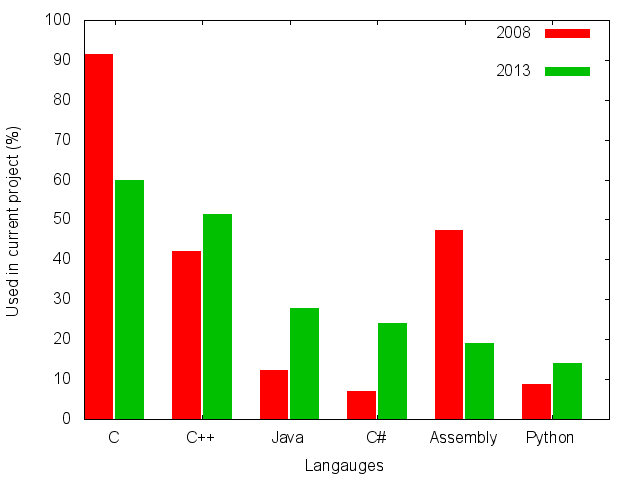
\includegraphics[scale=0.5]{figures/plots/langs.png}
  \end{center}
  \caption{}
  \label{fig:vdc:langs}
\end{figure}


VDC Research indicate that the portion of embedded systems design projects powered by Java rose from 12.3 percent in 2008 to 27.8 percent in 2013. Meanwhile, use of C during the same period dropped from 91.6 percent to 59.8 percent, and use of Assembly fell from 47.4 percent to 19.1 percent.



Embed, Arduino
Raspberry PI, Tessel
RTOS, Linux, Barebone
